\chapter{Opis doświadczenia}
\label{cha:dos}
Przeprowadzone doświadczenie polega na porównaniu dostępnych w środowisku Microsoft Azure algorytmów klasyfikacji danych dwuklasowych wraz z algorytmem stworzonym na potrzeby pracy inżynierskiej o tytule ,,\textit{Wykorzystanie algorytmów genetycznych w systemach wykrywania intruzów w sieciach komputerowych}''~\cite{Blyszcz2022} oraz z algorytmem DANet~\cite{Chen2022}.\ Doświadczenie przebiegało według \refsource{schematu}{fig:sch-prac}.

\begin{figure}[H]
    \centering
    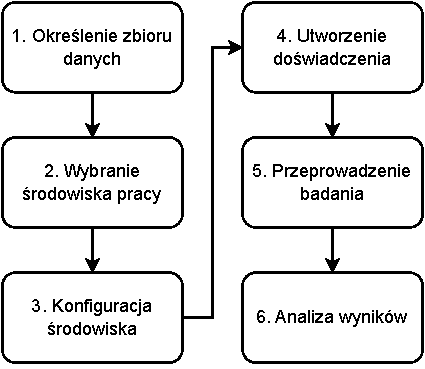
\includegraphics[width=0.9\textwidth]{images/schemat_pracy}
    \captionsource{Schemat przebiegu doświadczenia}{Opracowanie własne}
    \label{fig:sch-prac}
\end{figure}

\vfill
\pagebreak

\section{Założenie techniczne}

Dane prezentowane w \refsource{Tabeli}{tab:technical} określają podstawowe założenia techniczne przyjęte w trakcie wykonywania analizy porównawczej.\ Dane te dotyczą między innymi środowiska, w którym wykonane było doświadczenie.\ Dodatkowo uwzględniono zestaw danych oraz biblioteki użyte w trakcie tworzenia doświadczenia.

\begin{table}[H]
    \centering
    \captionsource{Założenia techniczne pracy dyplomowej}{Opracowanie własne}
    \label{tab:technical}
    \begin{tabular}{|l|l|}
        \hline
        \textbf{Środowisko uruchomieniowe} & Machine Learning Studio\cite{azureml} \\ \hline
        \textbf{Język programowania} & Python 3.x \\ \hline
        \multirow{3}*{\textbf{Wykorzystane biblioteki}} & scikit-learn~\cite{scikit-learn} \\
        \cline{2-2}
        & Numpy~\cite{Harris2019} \\
        \cline{2-2}
        & Pandas~\cite{pandas, McKinney2010} \\
        \hline
        \textbf{Wykorzystane dane} & CICDS2017~\cite{cicds2017kaggle} \\
        \hline
    \end{tabular}
\end{table}

\section{Dane}
\label{sec:data}
Zbiór danych został przygotowany przez Kanadyjski Instytut Cyberbezpieczeństwa działający przy Uniwersytecie Nowy Brunszwik.\ Został wykonany za pomocą narzędzia CICFlowMeter
~\cite{Ahlashkari2022}.\ Zbiór zawiera 79 cech ruchu sieciowego, do których zaliczyć można:
\begin{enumerate}
    \item etykietę,
    \item czas trwania przesyłu,
    \item minimalną długość pakietu zwrotnego,
    \item maksymalną długość pakietu zwrotnego,
    \item port docelowy,
    \item długość pakietów.
\end{enumerate}
Zbiór pozwala na określenie czy ruch sieciowy jest życzliwy \trans{ang. BENING}, czy nieżyczliwy (różne możliwe formy ataku na sieć).\ Dodatkowo zbiór został podzielony na pięć dni roboczych: poniedziałek 3.07.2017 - piątek 7.07.2017.\ Dane z poniedziałku zawierają jedynie ruch życzliwy.\ W pozostałe dni zostały zasymulowane ataki na sieć komputerową~\cite{Blyszcz2022, unbkaggle}.

\section{Programistyczne środowisko badawcze}
Jako środowisko programistyczne zostało wybrane Azure Machine Learning Studio.\ Zostało to spowodowane możliwością uniezależnienia obliczeń od komputera lokalnego.\ Platforma umożliwia łatwy sposób na tworzenie skomplikowanych potoków zadań, które składają się z komponentów wielokrotnego użytku.\ Każdy komponent uruchamia się w środowisku odizolowanym od pozostałych operacji.\ Dzieje się tak dzięki wykorzystaniu wielowęzłowych klastrów obliczeniowych, bazujących na oprogramowaniu Docker.\ Klastry te mogą skalować się w zależności od potrzeb oraz dostępnej jednostki~\cite{MicrosoftLearn2023}.
\\ \\
Całe doświadczenie zostało odwzorowane w graficznym potoku narzędzia ,,\textit{Projektant}'' oraz przedstawione na \refsource{zdjęciu}{fig:pipeline}.

\begin{landscape}
    \centering
\begin{figure}[H]
    \centering
    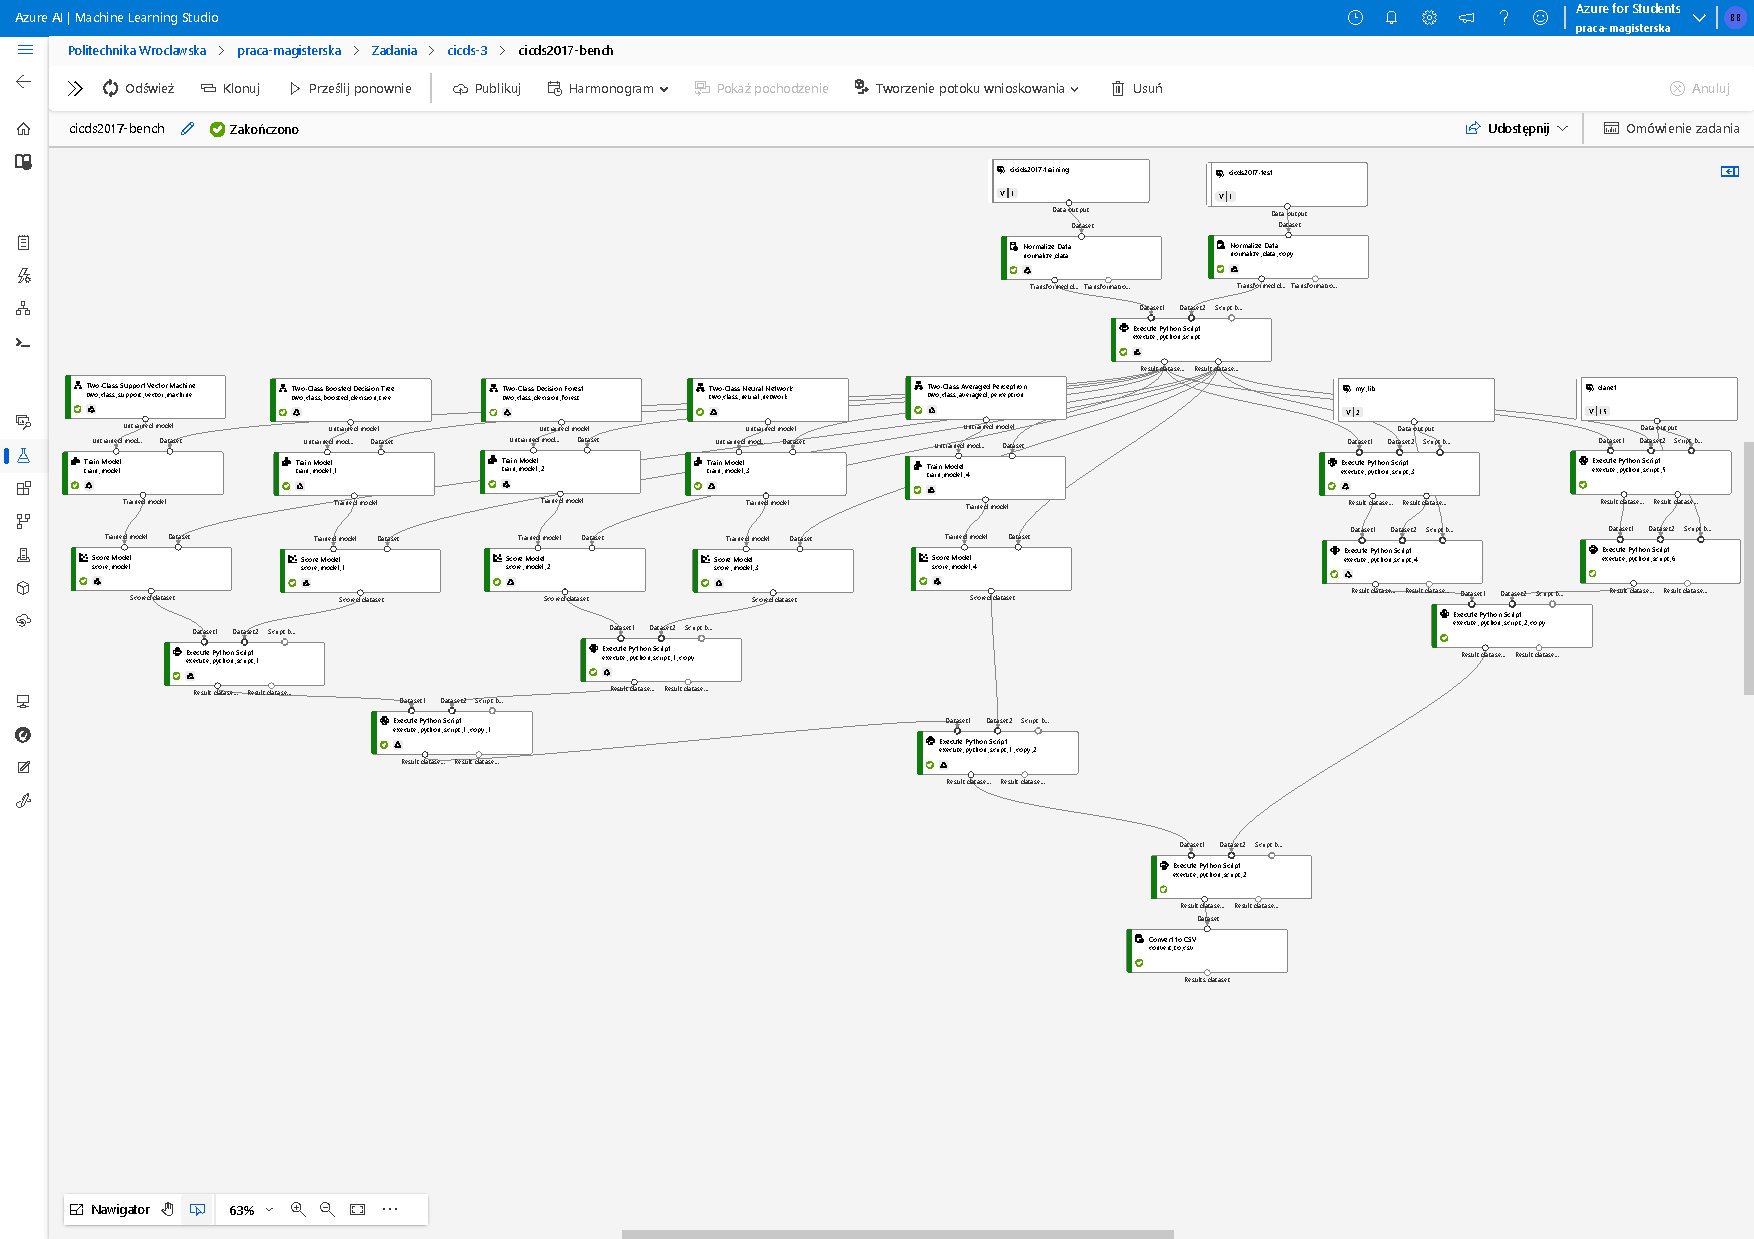
\includegraphics[height=0.9\textwidth]{images/pipeline}
    \captionsource{Potok zadań}{Opracowanie własne}
    \label{fig:pipeline}
\end{figure}
\end{landscape}

\section{Algorytmy wykorzystane w doświadczeniu}
\label{sec:alg}
W trakcie eksperymentu zastosowano różne algorytmy klasyfikacji danych.\ Charakterystyczną cechą tych algorytmów jest klasyfikacja ukierunkowana na 2 kategorie wejściowe.\ W tym wypadku są to kategorie ruchu sieciowego: [\textbf{BENIGN} \trans{pl. życzliwy}, \textbf{OTHER} \trans{pl. inne}], gdzie inne to pozostałe typy ruchu sieciowego.

\subsection{Two-Class Support Vector Machine}
Algorytm SVM ma za zadanie znaleźć hiperpłaszczyznę w przestrzeni K-wymiarowej (K - liczba cech), która rozdziela zbiory punktów odpowiadających różnym klasom.\ W pierwszej kolejności szuka się separatora między klasami, a następnie przekształca się dane w taki sposób, by można przekształcić separator w hiperpłaszczyznę~\cite{IBM}.\ Sposób działania został zobrazowany za pomocą \refsource{wykresów}{fig:svm-schem}.\ Część \refsource{potoku}{fig:pipeline} odpowiedzialnego za SVM to \refsource{schemat}{fig:svm-pipe}.

\begin{figure}[H]
    \begin{subfigure}[m]{0.45\textwidth}
        \centering
        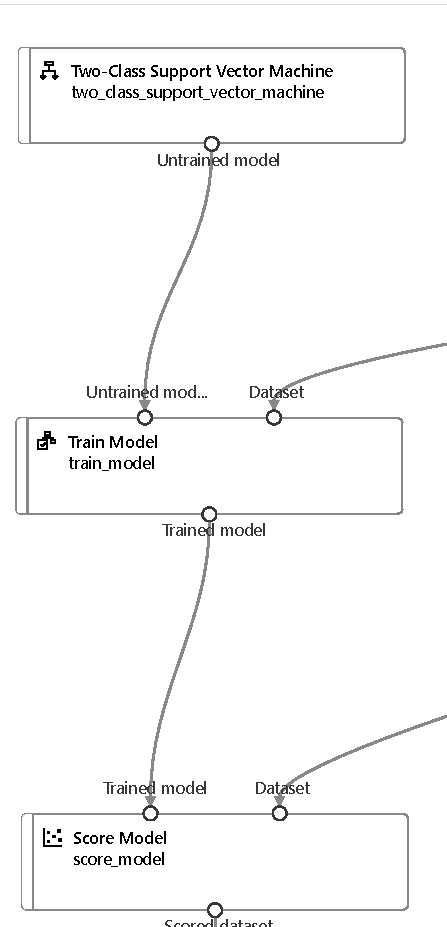
\includegraphics[width=\textwidth]{images/svm_pipe}
        \captionsource{Potok zadań dla modelu \textit{Two-Class Support Vector Machine}}{Opracowanie własne}
        \label{fig:svm-pipe}
    \end{subfigure}
    \hfill
    \begin{subfigure}[m]{0.45\textwidth}
        \centering
        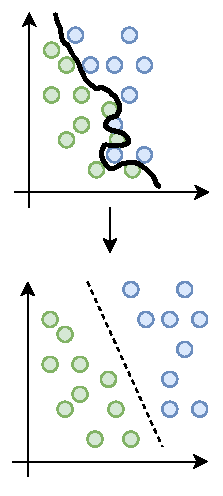
\includegraphics[width=\textwidth]{images/svm}
        \captionsource{Schemat SVM}{\cite{Statsoft}}
        \label{fig:svm-schem}
    \end{subfigure}
\end{figure}

\vfill
\pagebreak

\subsection{Two-Class Boosted Decision Tree}
Jest to algorytm drzewa decyzyjnego oparty o algorytm LightGBM.\ Dzięki zastosowaniu tego podejścia algorytm oparty o drzewo decyzyjne działa szybciej oraz ma mniejszą złożoność obliczeniową.\ Algorytm ten działa na zasadzie doboru odpowiedniego liścia, zamiast jak w przypadku klasycznych algorytmów opartych na drzewie, wyboru odpowiedniej warstwy~\cite{LightGBM}.\ Sposób podejścia liściastego został ukazany na \refsource{schemacie}{fig:leaf}.\ Model wykorzystywany w Azure ML został ukazany na \refsource{rysunku}{fig:dt-pipe}.
\begin{figure}[H]
    \begin{subfigure}[m]{0.3\textwidth}
        \centering
        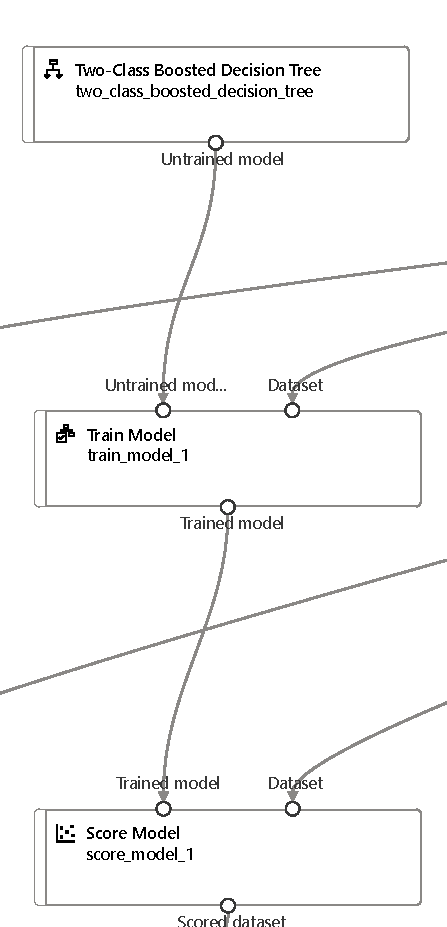
\includegraphics[width=\textwidth]{images/dt_pipe}
        \captionsource{Potok zadań dla modelu \textit{Two-Class Boosted Decision Tree}}{Opracowanie własne}
        \label{fig:dt-pipe}
    \end{subfigure}
    \hfill
    \begin{subfigure}[m]{0.66\textwidth}
        \begin{subfigure}[m]{\textwidth}
            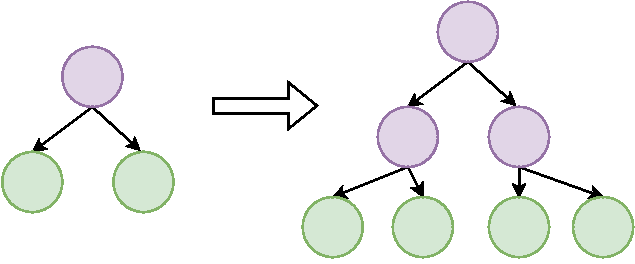
\includegraphics[width=\textwidth]{images/level-wise}
        \end{subfigure}
        \begin{subfigure}[m]{\textwidth}
            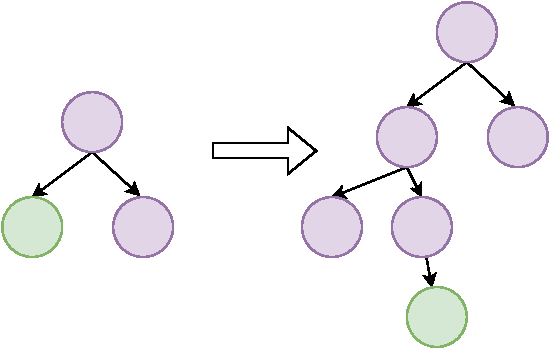
\includegraphics[width=\textwidth]{images/leaf-wise}
        \end{subfigure}
        \captionsource{Sposób działania algorytmu}{\cite{LightGBM}}
        \label{fig:leaf}
    \end{subfigure}
\end{figure}
\vfill
\pagebreak

\subsection{Two-Class Decision Forest}
Las decyzyjny to algorytm, którego wynik opiera się o agregację wyników wielu drzew decyzyjnych.\ Uzyskanie wyniku zależy od algorytmu trenowania lasu.\ Przykładowo w klasyfikacji losowym lasem wieloklasowym \trans{ang. Multi-class random forest classification}, każde drzewo głosuje na jedną klasę.\ Klasa, która zostanie wybrana większością głosów, zostaje uznana za wynikową~\cite{Google}.\ Model wykorzystany w Azure ML pokazano na \refsource{modelu}{fig:df-pipe}

\begin{figure}[H]
    \centering
    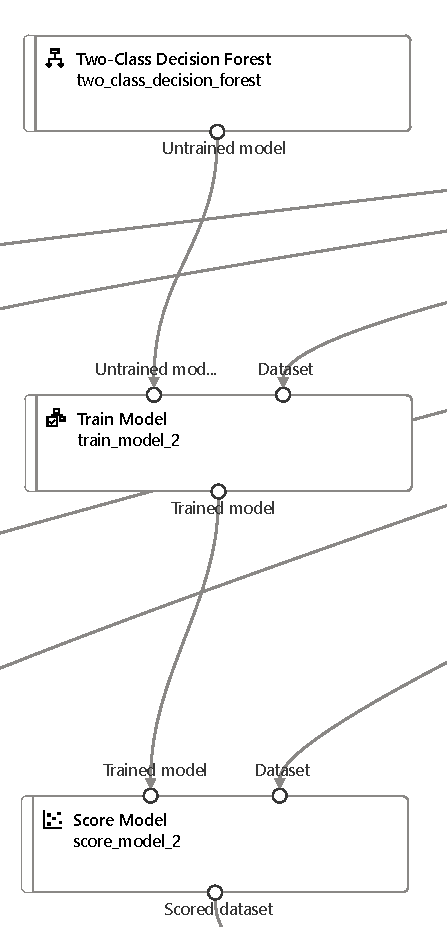
\includegraphics[width=0.3\textwidth]{images/df_pipe}
    \captionsource{Potok zadań dla modelu \textit{Two-Class Decision Forest}}{Opracowanie własne}
    \label{fig:df-pipe}
\end{figure}

\vfill
\pagebreak

\subsection{Two-class Neural Network}
Jest to sieć neuronowa, która składa się z warstwy wejściowej, trzech warstw ukrytych (każda posiada po 100 węzłów), oraz z warstwy wyjściowej.\ Przykładowa sieć neuronowa została zobrazowana na \refsource{schemacie}{fig:neural-network}.\ Moduł wykorzystany w Azure ML ukazano na \refsource{rysunku}{fig:nn-pipe}.

\begin{figure}[H]
    \centering
    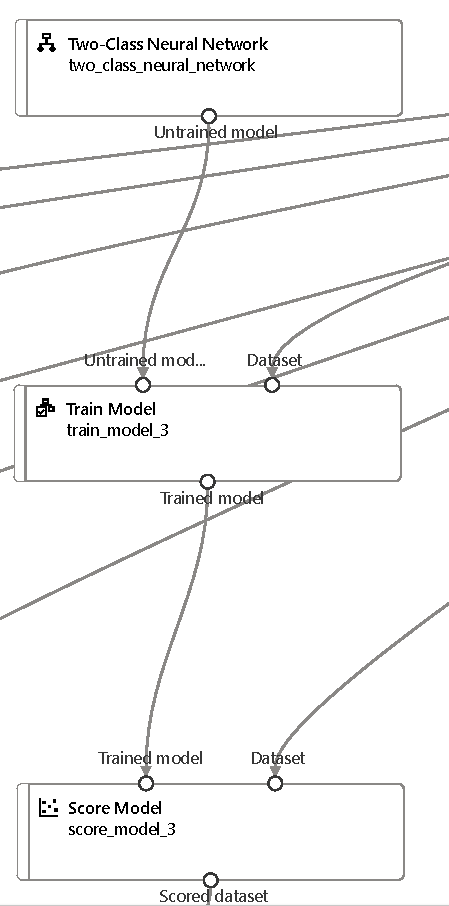
\includegraphics[width=0.3\textwidth]{images/nn_pipe}
    \captionsource{Potok zadań dla modelu \textit{Two-Class Neural Network}}{Opracowanie własne}
    \label{fig:nn-pipe}
\end{figure}

\vfill
\pagebreak

\subsection{Two-Class Average Perceptron}
Jest to najprostsza odmiana sieci neuronowej, czyli pojedynczy perceptron, który jest matematycznym modelem neuronu.\ Składa się on z \textit{n} wejść, takiej samej ilości wag, progu $\Theta$, sumatora, funkcji aktywującej i wyjścia.\ Został zobrazowany na \refsource{schemacie}{fig:neuron}.\ Może służyć za prosty klasyfikator binarny albo za regresor.\ Model wykorzystany w Azure ML ukazano na \refsource{zdjęciu}{fig:ap-pipe}.

\begin{figure}[H]
    \centering
    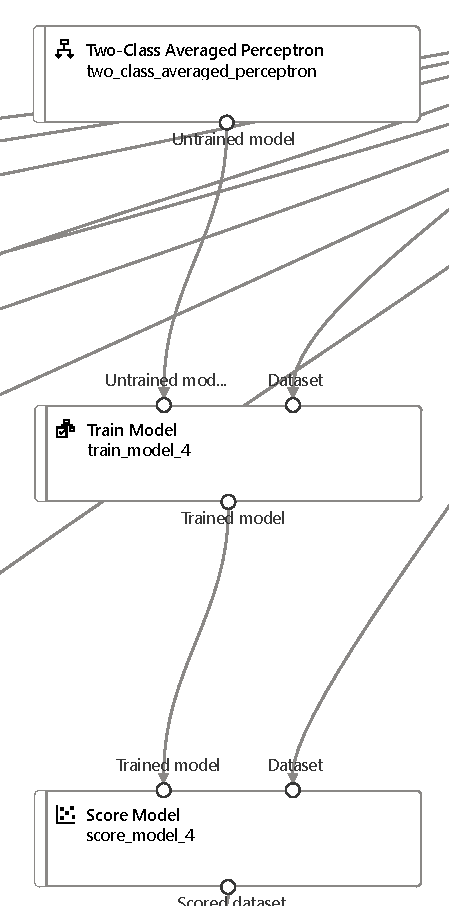
\includegraphics[width=0.3\textwidth]{images/ap_pipe}
    \captionsource{Potok zadań dla modelu \textit{Two-Class Average Perceptron}}{Opracowanie własne}
    \label{fig:ap-pipe}
\end{figure}

\vfill
\pagebreak

\subsection{Gausian Naive Bayes - with GA}
Algorytm ten polega na połączeniu algorytmu genetycznego (GA) wraz z klasyfikatorem naiwnym Bayesa wykorzystującego rozkład Gaussa (GNB).\ Zadaniem algorytmu genetycznego jest znalezienie najistotniejszych cech w zbiorze tabelarycznym.\ Poszukiwane cechy powinny pozwolić na zmniejszenie wymiarowości danych oraz na zmniejszenie kosztów obsługi samego klasyfikatora.\ Co może zostać uzyskane późniejszych etapach testowania, ze względu na zmniejszoną ilość danych wymaganych do przetworzenia.\ GA wykorzystywał w metodzie \textbf{fitness} algorytm GNB w celu określenia dopasowania danych.\ Zadaniem GNB było znalezienie najlepszej dostępnej kombinacji cech, które pozwalały na uzyskanie najlepszego dopasowania~\cite{Blyszcz2022}.\ Model wykorzystywany w Azure ML różni się od gotowych modeli tym, że dołączono do niego bibliotekę napisaną w języku Python, która zawiera kod wykorzystywany w pracy inżynierskiej autora~\cite{Suvres2023}.
\begin{figure}[H]
    \centering
    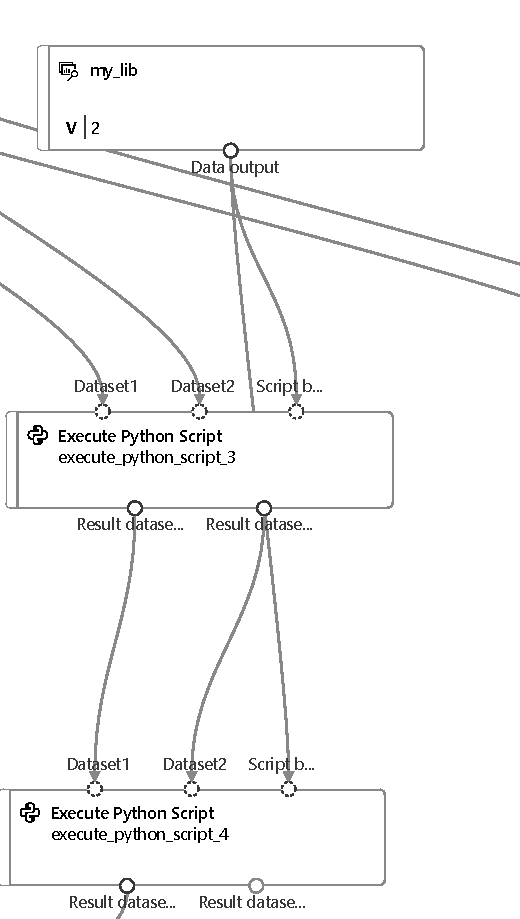
\includegraphics[width=0.3\textwidth]{images/ga_pipe}
    \captionsource{Potok zadań dla modelu}{Opracowanie własne}
    \label{fig:ga-pipe}
\end{figure}

\vfill
\pagebreak

\subsection{DANet}
Twórcy tego algorytmu wprowadzają dodatkową warstwę abstrakcyjną o nazwie ,,\textit{Abstract Layer}''.\ Warstwy te budują sieć o nazwie ,,\textit{Deep Abstract Network}'' (DANet).\ Zadanie dodatkowych warstw jest grupowanie cech w skorelowanych zbiorach.\ Zbiory te budują sieć powiązań między sobą w formie sieci semantycznej.\ Gdy sieć semantyczna jest zbudowana, to w ostatnim kroku wykonywana jest klasyfikacja w trzywarstwowej sieci perceptronów \trans{ang. Multilayer Perceptron network} (MLP)~\cite{Chen2022, Danet}.\ Model znajdujący się z Azure ML został przedstawiony na \refsource{zdjęciu}{fig:danet-pipe}, zaś sposób działania ukazano na \refsource{schematach}{fig:danet-abst}.

\begin{figure}[H]
    \begin{subfigure}[m]{0.49\textwidth}
        \centering
        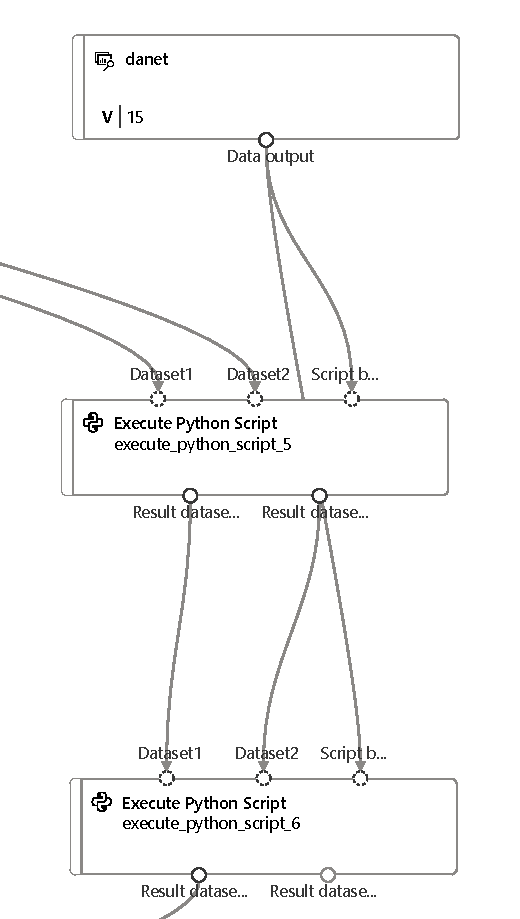
\includegraphics[width=0.4\textwidth]{images/danet}
        \captionsource{Potok zadań dla modelu \textit{DANet}}{Opracowanie własne}
        \label{fig:danet-pipe}
    \end{subfigure}
    \hfill
    \begin{subfigure}[m]{0.49\textwidth}
        \begin{subfigure}[m]{\textwidth}
            \centering
            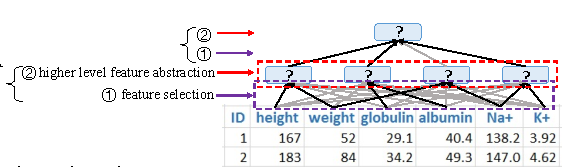
\includegraphics[width=\textwidth]{images/danet_1}
        \end{subfigure}
        \begin{subfigure}[m]{\textwidth}
            \centering
            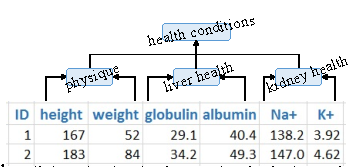
\includegraphics[width=\textwidth]{images/danet_2}
        \end{subfigure}
        \captionsource{Sposób działania DANet}{\cite{Chen2022}}
        \label{fig:danet-abst}
    \end{subfigure}

\end{figure}




